
\chapter{Descripción del Trabajo}
\label{cap:descripcionTrabajo}
En este capitulo se describe el framework de enemigos creado, mediante el diseño de componentes más sencillos. 
Primero se describirá el contexto y por tanto la utilidad de la herramienta, aquí se detallaran juegos analizados y sus características en común. Después se explicará que elementos la componen y por último se detallarán algunos ejemplos de uso. \\
\section{Contexto}
Como se señala en  \citet{Build_a_Bad_Guy_Workshop}, los enemigos bien diseñados son clave para evitar que los niveles queden planos y, en consecuencia, aburridos para el jugador.
Un buen diseño de enemigos va más allá de poner un obstáculo en el camino. Aporta dinamismo, construye la atmósfera del juego y hasta cuenta parte de la historia. Un enemigo puede obligarte a pensar una estrategia específica para vencerlo, o incluso tener una personalidad y comportamientos complejos que hacen que el enfrentamiento sea más significativo e inmersivo. En definitiva, diseñar a los antagonistas es una parte fundamental para crear un juego que enganche y deje huella.

\subsection{Enemigo}
Los enemigos son entidades programadas para enfrentarse al jugador y crear desafíos dentro del juego. Su diseño incluye características, comportamientos y habilidades diseñadas para interactuar con las mecánicas del juego y contribuir a la experiencia del jugador. \\
\subsection{Análisis de enemigos en videojuegos}
El análisis de diversos documentos muestra que la mejor forma de hacer que un enemigo destaque y de un gran potencial al juego es que tenga unos comportamientos únicos. Estos comportamientos han ido evolucionando con el tiempo volviéndose cada vez más sofisticados. Cada enemigo se define mediante una forma única de un conjunto de componentes bien seleccionados que permiten identificarlo y recordarlo.
Con dicha sofisticación, ha aumentado la complejidad del trabajo en el diseño. Para solucionarlo hemos propuesto una herramienta con la composición indicada a continuación.

\section{Composición}
En este trabajo, se ha decidido entender como enemigo a cualquier entidad que pueda repercutir de forma negativa en el jugador, esto significa que no se limita el concepto de enemigo a figuras típicas, como monstruos o soldados hostiles, sino que se amplía su definición a toda entidad que suponga un riesgo, dificultad o amenaza para el progreso o el bienestar del jugador dentro del juego, como pueden ser pinchos, lava o gotas de ácido.
Además separamos cada enemigo por comportamientos diferentes, implicando que elementos que clásicamente aparecen en conjunto, como la tubería y la gota de ácido o la bala y el pistolero, serán considerados como dos enemigos distintos.\\

\subsection{Máquina de estados finita}

La Máquina de Estados Finita (FSM, Finite State Machine) es el núcleo de la lógica que define el comportamiento de los enemigos en nuestro diseño. Cada enemigo tiene su propia FSM, configurada específicamente para representar sus patrones de acciones, reacciones y relaciones en el juego. La FSM organiza el comportamiento de los enemigos mediante estados y transiciones:
Los estados agrupan las acciones que el enemigo puede realizar en un momento dado.
Las transiciones permiten cambiar de un estado a otro y son activadas por sensores y emisores.\\

\begin{figure}[!h]
	\centering
	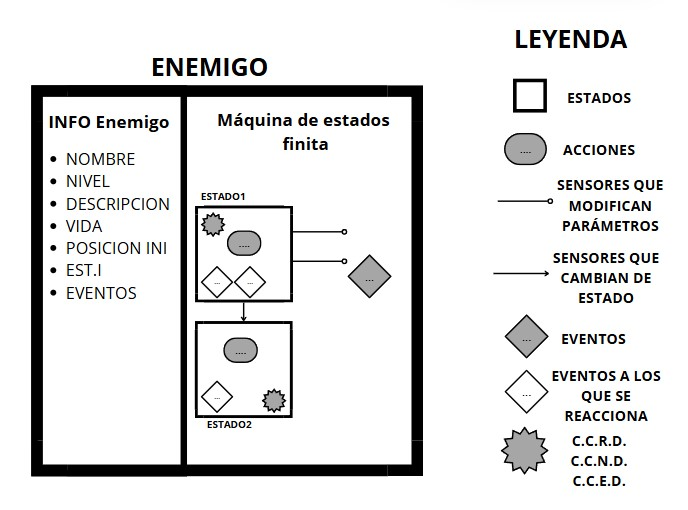
\includegraphics[height=5cm]{Imagenes/EnemigoGeneral.png}
	\caption{Enemigo General }
	\label{fig:EnemigoGeneral}
\end{figure}
Estos conceptos (\hyperref[subsec:estado]{estados}, \hyperref[subsec:acciones]{acciones}, \hyperref[subsec:sensores y emisores]{sensores y emisores}) se desarrollan con mayor detalle en los apartados siguientes.

\subsection{Estado}
\label{subsec:estado}

Dentro del marco de la Máquina de Estados Finita (FSM), un estado se define como un conjunto específico de acciones y la potencial activación de mecanismos de percepción (sensores) y de emisión de señales (emisores). Esta conjunción de elementos define de manera integral la conducta observable del enemigo en un momento dado. Las acciones que un estado puede englobar comprenden uno o varios tipos de movimiento que resulten compatibles entre sí, permitiendo una ejecución coordinada de desplazamientos. Adicionalmente, un estado puede tener la capacidad de generar nuevas entidades enemigas a través de un mecanismo de instanciación (spawner), enriqueciendo la dinámica y la complejidad del entorno de juego.

\subsection{Actuadores (Acciones)}
\label{subsec:acciones}
Hace referencia a un conjunto de movimientos y habilidades que definen lo que un enemigo puede hacer en el videojuego. Esto incluye distintos tipos de desplazamientos y la capacidad de crear otros enemigos de forma independiente mediante spawners. Estas habilidades no siempre son compatibles entre sí, teniendo una tabla en la que se indicaran las relaciones entre ellas. Además no es necesario utilizar siempre todas las acciones de forma que a veces un enemigo podrá realizar un tipo de movimiento o usar un spawner de manera exclusiva, mientras que en otras podrá combinar varias habilidades según su diseño y complejidad. Esto permite adaptar las capacidades de los enemigos para diferentes situaciones en el juego.
\subsubsection{Spawner}
Capacidad que poseen los enemigos para generar otros enemigos independientes, es decir, poder crear nuevas unidades que actúan de forma autónoma dentro del juego.\\
Los spawners presentan características únicas dentro del sistema de enemigos, ya que su objetivo no es solo enfrentarse al jugador, sino también aumentar el número de amenazas de manera continua o en función de ciertas condiciones.
Implementar un spawner requiere establecer ciertas reglas de generación de enemigos, tales como la frecuencia de aparición, el número máximo de enemigos generados o si las unidades generadas son temporales o persistentes.
\subsubsection{Movimiento}
Podemos definir el término movimiento como el desplazamiento o cambio de posición de un enemigo dentro del juego. Sin embargo, el concepto de movimiento también puede aplicarse en el caso de enemigos que permanecen en una posición fija, haciendo referencia a la ausencia de éste. Los movimientos son fundamentales para definir el comportamiento de los personajes, ya que permiten la interacción con el jugador y el entorno.\\
A continuación se muestran todos los movimientos implementados, junto con una breve descripción.
\begin{itemize}
  \item \textbf{Horizontal Actuator}: Desplaza el objeto horizontalmente, hacia la izquierda o derecha.
    \item \textbf{Vertical Actuator}: Desplaza el objeto verticalmente, hacia arriba o abajo.
    \item \textbf{Directional Actuator}: Mueve el objeto en una dirección definida por un ángulo.
    \item \textbf{Circular Actuator}: Hace que el objeto siga un movimiento circular alrededor de un punto.
    \item \textbf{Move To A Point Actuator}: Dirige el objeto hacia puntos aleatorios dentro de un área o puntos predefinidos.
    \item \textbf{Move To An Object Actuator}: Desplaza el objeto hacia una entidad que puede estar en movimiento.
    \item \textbf{Spline Follower Actuator}: Permite al objeto seguir una trayectoria definida por un spline.
\end{itemize}
\subsubsection{Compatibilidad}
La versatilidad de la herramienta se potencia al permitir la combinación de diversos actuadores simultáneamente. En este sentido, un enemigo podría perfectamente desplazarse horizontalmente mientras activa un spawner para generar secuaces. Esta sinergia entre actuadores (movimientos y spawners) enriquece la complejidad del comportamiento y abre un abanico de posibilidades creativas para los diseñadores.\\
No obstante, es crucial reconocer que no todas las combinaciones de acciones resultan coherentes o deseables desde la perspectiva del diseño del juego. Por ejemplo, intentar realizar un movimiento vertical mientras se está definido un movimiento circular podría generar comportamientos visuales o de jugabilidad no intencionados. \\
Para clarificar estas interdependencias y asegurar la coherencia en la configuración de los enemigos, se ha elaborado la tabla \textbf{tabla~\ref{tab:compatibilidad}} de compatibilidad. Esta tabla actuará como una guía visual e intuitiva, indicando qué combinaciones de movimientos y la activación de spawners son factibles y recomendadas, permitiendo a los diseñadores construir enemigos con comportamientos complejos pero lógicos y bien definidos.

\begin{table}[!h]
    \centering

    \renewcommand{\arraystretch}{1.5}
    \setlength{\tabcolsep}{4pt} % Reduce el espacio entre columnas
    \resizebox{\textwidth}{!}{
        \begin{tabular}{c|cccccc}
            & \cellcolor{gray!60} Movimiento Horizontal & \cellcolor{gray!60} Movimiento Vertical & \cellcolor{gray!60} Quieto & \cellcolor{gray!60} Movimiento hacia un punto & \cellcolor{gray!60} Circular/Rotación & \cellcolor{gray!60} Péndulo \\
            \hline
            \cellcolor{gray!40} Movimiento Horizontal &  &  &  &  &  &  \\ \addlinespace
            \cellcolor{gray!40} Movimiento Vertical & \cellcolor{green!70} &  &  &  &  &  \\ \addlinespace
            \cellcolor{gray!40} Quieto & \cellcolor{red!70} & \cellcolor{red!70} &  &  &  &  \\ \addlinespace
            \cellcolor{gray!40} Movimiento hacia un punto & \cellcolor{green!70} & \cellcolor{green!70} & \cellcolor{red!70} &  &  &  \\ \addlinespace
            \cellcolor{gray!40} Circular/Rotación & \cellcolor{green!70} & \cellcolor{green!70} & \cellcolor{red!70} & \cellcolor{green!70} &  &  \\ \addlinespace
            \cellcolor{gray!40} Péndulo & \cellcolor{green!70} & \cellcolor{green!70} & \cellcolor{red!70} & \cellcolor{green!70} & \cellcolor{green!70} &  \\ \addlinespace
        \end{tabular}
    }
    \caption{Matriz de compatibilidad de movimientos}
    \label{tab:compatibilidad}
\end{table}


\subsection{Sensores y Emisores}
\label{subsec:sensores y emisores}
Los términos sensores y emisores definen los mecanismos mediante los cuales los personajes interactúan con su entorno y entre sí.
Podemos definir el término sensor como el elemento necesario para medir variables exteriores y enviar la información al enemigo.\\
Definimos emisor como anónimo de sensor, es decir, es aquel elemento que envía información del enemigo al exterior.
A continuación se enumerarán los diferentes sensores y emisores disponibles en la herramienta.
\begin{itemize}
    \item \textbf{Area Sensor}: Detecta si un objeto entra o sale en una zona de detección.
    \item \textbf{Collision Sensor}: Detecta colisiones físicas con otros objetos.
    \item \textbf{Distance Sensor}: Detecta si un objeto está dentro o fuera de una distancia específica.
    \item \textbf{Time Sensor}: Detecta cuando ha transcurrido un tiempo determinado.
    \item \textbf{Damage Sensor}: Detecta si el objeto ha recibido daño.
    \item \textbf{Damage Emitter}: Aplica daño a entidades con Damage Sensor.
\end{itemize}
\subsection{Daño}
Aunque ya ha aparecido el concepto de daño en los sensores y emisores creados, es importante definir con precisión su significado así como las diversas formas de daño existen. \\
Es relevante mencionar que al hablar de daño, el concepto de enemigo pierde relevancia y se aborda más con respecto a las representaciones físicas de volúmenes de colisión.\\
Se define daño como la consecuencia negativa que recibe una entidad con respecto a su vida. Esto se produce como la consecuencia de que un volumen de colisión que emite daño colisione contra otro volumen de colisión que recibe daño.\\
Existen diferentes tipos de daño y parámetros específicos que determinan cómo los volúmenes de colisión reciben, emiten y procesan daño.
La primera consideración que hay que tener en cuenta es que el daño no es bidireccional, lo que implica que un volumen que recibe daño no tiene porqué emitir daño. Para reflejar esta diferenciación, se pueden distinguir tres tipos de cajas:
\begin{itemize}
	 \item \textbf{Caja de Colisión Recibir Daño:} Áreas en las que el enemigo es vulnerable.
	 \item \textbf{Caja de Colisión Emitir Daño:} Áreas desde las que el enemigo inflige daño.
	 \item  \textbf{Caja de Colisión No Daño:} Zonas invulnerables del enemigo que no interactúan con el sistema de daño.
\end{itemize}
Aunque en teoría distinguimos esos tres tipos, a la hora de implementar son cosas distintas. Las cajas de no daño son áreas sin ningún elemento añadido. Las que reciben daño llevan el componente llamado Damage Sensor que detecta y gestiona el daño. Las que dan daño tienen un Damage Emitter que se encarga de hacer daño a otros.

Además, se puede distinguir entre tres tipos de daños:
\begin{itemize}
    \item \textbf{Instantáneo:} Aplica daño una única vez el daño al tener contacto.
    \item \textbf{De Permanencia:} Inflige daño continuo mientras haya contacto, definiendo la cantidad y la frecuencia de aplicación de daño.
    \item \textbf{Residual:} Aplica daño inicial y luego daño periódico tras el contacto, definiendo cantidades, frecuencia de aplicación y número de aplicaciones.
\end{itemize}

